\chapter{\textbf{Optimization of communication}}



\textbf{Optimization of communication}

There are two factors to optimize the communication.\cite {Anna and Bob}

\begin{itemize}
  \item Effective communication means getting message across
  \item Optimization of information under constrains
\end{itemize}



These points can be achieved by applying Jean Iuc'c laws

First law:

\begin{figure}
  % Requires \usepackage{graphicx}
  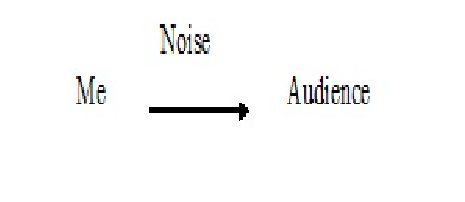
\includegraphics[width=4in]{law1.eps} 
  \caption {First Law}\label{2.1}  
\end{figure}

\begin{figure}
  % Requires \usepackage{graphicx}
  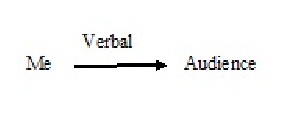
\includegraphics[width=4in]{law2.eps}
  \caption {Second Law}\label{2.2}
\end{figure}





The noise ie.anything that destroys the information.

In research presentation logo, too much of color and special effects etc.destroys the information.
It is like signal to noise ratio. So it is better to maximize the signal to noise ratio for good research presentation

The second law tells that optimization of information under constrain can be achieved by showing stand alone slides. The slides should be prepared  for audience not for speaker.



These two laws can be achieved by considering following points for good presentation.\cite {Stephen Moffat}

\begin{itemize}
  \item Be consistent. Ensure that all slides have the same or similar background images and color schemes. MS Power Point's design templates can be used for this.
  \item Prepare slides that use a bold color contrast, e.g. black or deep blue text on a cream background (black and white can be too glaring for the audience).
  \item Create bullet points which are clear summaries of key points. It is not necessary for bullet points to be complete sentences.
  \item Avoid using red or green for text or highlighting as it can be difficult to read
  \item Avoid using too much text. A useful guideline is the six-by-six rule (slides should have no more than six bullet points and each bullet point should be no more than six words long).
  \item Don't mix up your fonts and font sizes. Too many variations in font size and type can be visually confusing.
  \item Ensure that your text is at least 24pt otherwise it may be difficult to read on screen.
 \item Choose left align for all text to make it easier to read.
 \item Avoid multiple columns of text on a single slide as they can be difficult to follow on screen
 \item Use bold for a clear and simple form of emphasis and headings rather than UPPER CASE, italics or underlining
\item Set clear hierarchies for type size to help your audience distinguish between headings, main text and other types of text
\end{itemize}








